%%% Exemplo de utilização da classe ITA
%%%
%%%   por        Fábio Fagundes Silveira   -  ffs [at] ita [dot] br
%%%              Benedito C. O. Maciel     -  bcmaciel [at] ita [dot] br
%%%              Giovani Volnei Meinertz   -  giovani [at] ita [dot] br
%%%    	         Hudson Alberto Bode       -  bode [at] ita [dot]br
%%%    	         P. I. Braga de Queiroz    -  pi [at] ita [dot] br
%%%    	         Jorge A. B. Gripp         -  gripp [at] ita [dot] br
%%%    	         Juliano Monte-Mor         -  jamontemor [at] yahoo [dot] com [dot] br
%%%    	         Tarcisio A. B. Gripp      -  tarcisio.gripp [at] gmail [dot] com
%%%    	         
%%%
%%%  IMPORTANTE: O texto contido neste exemplo nao significa absolutamente nada.  :-)
%%%              O intuito aqui eh demonstrar os comandos criados na classe e suas
%%%              respectivas utilizacoes.
%%%
%%%  Tese.tex  2016-08-25
%%%  $HeadURL: http://www.apgita.org.br/apgita/teses-e-latex.php $
%%%
%%% ITALUS
%%% Instituto Tecnológico de Aeronáutica --- ITA, Sao Jose dos Campos, Brasil
%%%                   http://groups.yahoo.com/group/italus/
%%% Discussion list: italus {at} yahoogroups.com
%%%
%++++++++++++++++++++++++++++++++++++++++++++++++++++++++++++++++++++++++++++++
% Para alterar o TIPO DE DOCUMENTO, preencher a linha abaixo \documentclass[?]{?}
%   \documentclass[tg]{ita}			= Trabalho de Graduacao
%   \documentclass[tgfem]{ita}	= Para Engenheiras
%   								msc     		= Dissertacao de Mestrado
%   								mscfem   		= Para Mestras
%   								dsc      		= Tese de Doutorado
%   								dscfem   		= Para Doutoras
%   								quali    		= Exame de Qualificacao
%   								qualifem 		= Exame de Qualificacao para Doutoras
% Para 'Draft Version'/'Versao Preliminar' com data no rodape, adicionar 'dv':
%   \documentclass[dsc, dv]{ita} 
% Para trabalhos em Inglês, adicionar 'eng':
%   \documentclass[dsc, eng]{ita}
%		\documentclass[dsc, eng, dv]{ita}
%++++++++++++++++++++++++++++++++++++++++++++++++++++++++++++++++++++++++++++++

\documentclass[msc, dv]{ita}    % ITA.cls based on standard book.cls 
% Quando alterar a classe, por exemplo de [msc] para [msc, eng]) rode mais uma vez o botão BUILD OUTPUT caso haja erro
\usepackage{ae}
\usepackage{graphicx}
\usepackage{epsfig}
\usepackage{amsmath}
\usepackage{amssymb} 
\usepackage{subfig}
\usepackage{multirow}
\usepackage{float}
\usepackage{setspace}
%\usepackage{natbib}
%\usepackage[alf]{abntex2cite}
%++++++++++++++++++++++++++++++++++++++++++++++++++++++++++++++++++++++++++++++
% Espaçamento padrão de todo o documento
%++++++++++++++++++++++++++++++++++++++++++++++++++++++++++++++++++++++++++++++
\onehalfspacing

%singlespacing Para um espaçamento simples
%onehalfspacing Para um espaçamento de 1,5
%doublespacing Para um espaçamento duplo

%++++++++++++++++++++++++++++++++++++++++++++++++++++++++++++++++++++++++++++++
% Identificacoes (se o trabalho for em inglês, insira os dados em inglês)
% Para entradas abreviadas de Professora (Profa.) em português escreva: Prof$^\textnormal{a}$.
%++++++++++++++++++++++++++++++++++++++++++++++++++++++++++++++++++++++++++++++
\course{Física} % Programa de PG ou Curso de Graduação
\area{Ensino de Física} % Área de concentração na PG (Não utilizado no caso de TG)

% Autor do trabalho: Nome Sobrenome
\authorgender{masc}                     %sexo: masc ou fem
\author{Jefferson Rodrigues de}{Oliveira}
\itaauthoraddress{UnB - Campus Darcy Ribeiro - Asa Norte}{720910-900}{Brasília - DF - Brasil}

% Titulo da Tese/Dissertação
\title{Games digitais: uma abordagem de Física de Partículas Elementares no Ensino Médio}

% Orientador
\advisorgender{fem}                    % masc ou fem
\advisor{Prof.~Dr.}{Vanessa Carvalho de Andrade}{UnB}

% Coorientador (Caso não haja coorientador, colocar ambas as variáveis \coadvisorgender e \coadvisor comentadas, com um % na frente)
%\coadvisorgender{fem}									% masc ou fem
%\coadvisor{Prof$^\textnormal{a}$.~Dr$^\textnormal{a}$.}{Doralice Serra}{OVNI}

% Pró-reitor da Pós-graduação
%\bossgender{masc}												% masc ou fem
%\boss{Prof.~Dr.}{John von Neumann}

%Coordenador do curso no caso de TG
%\bosscoursegender{masc}									% masc ou fem
%\bosscourse{Prof.~Dr.}{John Walker}

% Palavras-Chaves informadas pela Biblioteca -> utilizada na CIP
\kwcip{Cupim}
\kwcip{Dilema}
\kwcip{Construção}

% membros da banca examinadora

\examiner{\itaadvisortitlebabel}{\itaadvisorname}{Presidente}{IF-UNB}
% Orientador(a)
\examiner{Prof. Dr.}{Mickey Mouse}{Membro interno vinculado ao programa}{IF-UNB}
\examiner{Prof. Dr.}{Richard Stallman}{Membro interno vinculado ao programa}{IF-UNB}
\examiner{Prof. Dr.}{Donald Duck}{Membro interno vinculado ao programa}{IF-UNB}
%\examiner{Prof. Dr.}{Mickey Mouse}{}{DISNEY}

% Data da defesa (mês em maiúsculo, se trabalho em inglês, e minúsculo se trabalho em português) 
\date{10}{01}{2017}

% Número CDU - (somente para TG)
\cdu{621.38}

% Glossario
\makeglossary
\frontmatter

\begin{document}

% Folha de Rosto e Capa para o caso do TG
\maketitle


% Dedicatoria: Nao esqueca essa secao  ... :-)
\begin{itadedication}
Aos amigos da Graduação e Pós-Graduação do ITA por motivarem tanto a criação deste template pelo Fábio Fagundes Silveira quanto por motivarem a mim e outras pessoas a atualizarem e aprimorarem este excelente trabalho.
\end{itadedication}

% Agradecimentos
\begin{itathanks}
Primeiramente, gostaria de agradecer ao Dr. Donald E. Knuth, por ter desenvolvido o \TeX.

Ao Dr. Leslie Lamport, por ter criado o \LaTeX, facilitando muito a utiliza��o do \TeX, e assim, eu n�o ter que usar o Word.

Ao Prof. Dr. Meu Orientador, pela orienta��o e confian�a depositada na realiza��o deste trabalho.

Ao Dr. Nelson D'�villa, por emprestar seu nome a essa importante via de tr�nsito na cidade de S�o Jos� dos Campos.

Ah, j� estava esquecendo... agrade�o tamb�m, mais uma vez ao \TeX, por ele n�o possuir v�rus de macro :-)

\end{itathanks}

% Epígrafe
\thispagestyle{empty}
\ifhyperref\pdfbookmark[0]{\nameepigraphe}{epigrafe}\fi
\begin{flushright}
\begin{spacing}{1}
\mbox{}\vfill
{\sffamily\itshape
``If I have seen farther than others,\\
it is because I stood on the shoulders of giants.''\\}
--- \textsc{Sir~Isaac Newton}
\end{spacing}
\end{flushright}

% Resumo
\begin{abstract}
\noindent
Aqui come�a o resumo do referido trabalho. N�o tenho a menor id�ia do que colocar aqui. Sendo assim, vou inventar. L� vai: Este trabalho apresenta uma metodologia de controle de posi��o das juntas passivas de um manipulador subatuado de uma maneira sub�tima. O termo subatuado se refere ao fato de que nem todas as juntas ou graus de liberdade do sistema s�o equipados com atuadores, o que ocorre na pr�tica devido a falhas ou como resultado de projeto. As juntas passivas de manipuladores desse tipo s�o indiretamente controladas pelo movimento das juntas ativas usando as caracter�sticas de acoplamento da din�mica de manipuladores. A utiliza��o de redund�ncia de atua��o das juntas ativas permite a minimiza��o de alguns crit�rios, como consumo de energia, por exemplo.
Apesar da estrutura cinem�tica de manipuladores subatuados ser id�ntica a do totalmente atuado, em geral suas carater�sticas din�micas diferem devido a presen�a de juntas passivas. Assim, apresentamos a modelagem din�mica de um manipulador subatuado e o conceito de �ndice de acoplamento. Este �ndice � utilizado na sequ�ncia de controle �timo do \mbox{manipulador}.
A hip�tese de que o n�mero de juntas ativas seja maior que o n�mero de
passivas  $(n_{a} > n_{p})$  permite o controle �timo das juntas passivas, uma vez que na etapa de controle destas h� mais entradas (torques nos atuadores das juntas ativas), que elementos a controlar (posi��o das juntas passivas). 
\end{abstract}

% Abstract
\begin{englishabstract}
\noindent

Well, the book is on the table. This work presents a control methodologie for the position of the  passive joints of an underactuated manipulator in a suboptimal way. The term underactuated refers to the fact that not all the joints or degrees of freedom of the system are equipped with actuators, which occurs in practice due to failures or as design result. The passive joints of manipulators like this are indirectly controlled by the motion of the active joints using the dynamic coupling characteristics. The utilization of actuation redundancy of the active joints allows the minimization of some criteria, like energy consumption, for example. Although the kinematic structure of an underactuated manipulator is identical to that of a similar fully actuated one, in general their dynamic characteristics are different due to the presence of passive joints. Thus, we present the dynamic modelling of an underactuated manipulator and the concept of coulpling index. This index is used in the sequence of the optimal control of the manipulator. Finish ok ok!

\end{englishabstract}

% Lista de figuras
\listoffigures %opcional

% Lista de tabelas
\listoftables %opcional

% Lista de abreviaturas
\listofabbreviations
\begin{longtable}{ll}
CTq & computed torque \\
DC & direct current \\
EAR & Equa��o Alg�brica de Riccati \\
GDL & graus de liberdade \\
ISR & interrup��o de servi�o e rotina \\
LMI & linear matrices inequalities \\
MIMO & multiple input multiple output \\
PD & proporcional derivativo \\
PID & proporcional integrativo derivativo \\
PTP & point to point \\
UARMII & Underactuated Robot Manipulator II \\
VSC & variable structure control \\

\end{longtable}

 %opcional

% Lista de simbolos
\listofsymbols
\begin{longtable}{ll}
$a$ & Dist�ncia\\
$\textbf{a}$ & Vetor de dist�ncias\\
$\textbf{e}_{j}$ & Vetor unit�rio de dimens�o $n$ e com o $j$-�simo componente igual a $1$ \\
$\textbf{K}$ & Matriz de rigidez\\
$m_1$ & Massa do cumpim\\
$\delta_{k-k_f}$ & Delta de Kronecker no instante $k_f$\\

\end{longtable}

 %opcional

% Sumario
\tableofcontents

\mainmatter
% Os capitulos comecam aqui

\chapter{Introdução}
\section{Objetivo}
O objetivo deste projeto de mestrado � desenvolver t�cnicas de controle sub�timo das juntas passivas (n�o atuadas) de um rob� subatuado, incluindo o estudo te�rico do tema, proposi��o de um m�todo de controle e sua verifica��o
experimental em um manipulador de tr�s graus de liberdade \cite{Nascimento1970}.

O teste \cite{Patagonios2001} e valida��o das t�cnicas de controle propostas foram realizados em um ambiente de simula��o e no manipulador
experimental, adquirido atrav�s do projeto FAPESP $N^{\circ}$ 98/00649-5, que se encontra em funcionamento no Laborat�rio de Sistemas Inteligentes (LASI) do Departamento de Engenharia El�trica da USP em S�o Carlos. Pode-se citar \cite{Furmento1995}:
\begin{itemize}
\item Isso;
\item Aquilo; e
\item Aquele outro.
\end{itemize}
\section{Motiva��o}
Manipuladores mec�nicos \cite{Sbornian2002} v�m sendo utilizados h� v�rias d�cadas para a automa��o de tarefas
repetitivas em ambientes industriais, ambientes estes de f�cil acesso tanto em termos f�sicos quanto em termos de baixo
risco � sa�de humana. Nos �ltimos anos, verifica-se uma utiliza��o cada vez maior de manipuladores em
ambientes de dif�cil acesso ou in�spitos, como no interior de usinas nucleares, no fundo dos oceanos e no
espa�o. A localiza��o dos manipuladores nesta nova gama de aplica��es faz com que sua manuten��o,
Dp�s uma falha mec�nica ou el�trica, seja custosa e demorada, portanto estes mecanismos requerem sofisticadas
metodologias de controle tolerante a falhas \cite{ITALUS2004}.

Ap�s a ocorr�ncia de uma falha em um de seus atuadores, o manipulador torna-se um sistema subatuado. Um sistema tamb�m pode se tornar subatuado quando � projetado  dessa maneira, ou quando o operador deliberadamente mant�m um ou mais atuadores dispon�veis inoperantes durante uma tarefa. Reduzindo o n�mero de atuadores sem reduzir o n�mero de graus de liberdade e ajustando-se o sistema de controle adequado, pode-se obter um mecanismo cujo consumo de energia � menor, mas cujas propriedades s�o mantidas \cite{Arystides1994}.

\begin{figure}[ht]
\centering
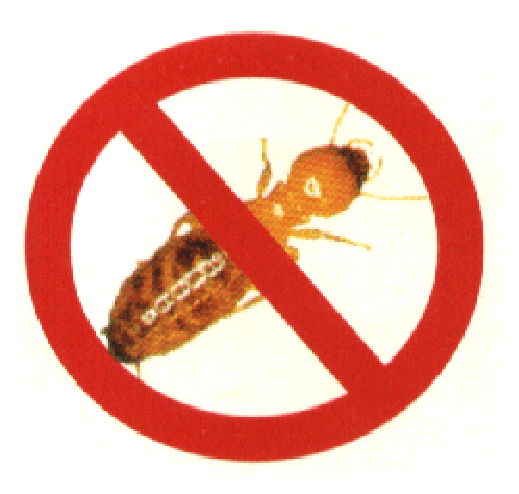
\includegraphics[width=0.5\textwidth]{Cap1/cupim}
\caption{Proibido estacionar cupins. Legenda grande, com o objetivo de demonstrar a indenta��o na lista de figuras.}
\label{cupim}
\end{figure}

Controle do manipulador ap�s uma falha � fundamental do ponto de vista de opera��o, principalmente nos casos descritos acima, em que a localiza��o do manipulador impede sua manuten��o de forma f�cil. Recentemente tem havido a combina��o
de algor�tmos de detec��o e isola��o de falhas com os de controle p�s-falha em um m�todo unificado. Uma extens�o desse trabalho, que v� o problema de controle tolerante a falhas atrav�s de uma perspectiva integrada, foi proposta por
{marcel4}. Os autores apresentam um ambiente h�brido consistindo de tr�s unidades b�sicas que garantem a complei��o de tarefas na presen�a de qualquer n�mero de juntas falhas (Figura \ref{cupim}). A primeira unidade � um esquema de detec��o
e isola��o de falhas que continuamente monitora o manipulador para detectar e identificar poss�veis falhas nas juntas. A segunda unidade � respons�vel pela reconfigura��o do controle. A terceira unidade � composta de algor�tmos de
controle apropriados para cada tipo de configura��o do rob�, baseado na informa��o da unidade de reconfigura��o \cite{COFFEE2000}.

No presente trabalho nos concentramos na unidade de algor�tmo de controle, e mais especificamente no problema de controle da posi��o  angular de uma junta falha para qualquer posi��o desejada de uma maneira sub�tima, quando dispomos
de redund�ncia de atua��o para a realiza��o dessa tarefa. O termo sub�timo se deve ao fato de que n�o h� garantias de otimalidade em vista das n�o-linearidades inerentes ao sistema e de outros fatores que ser�o abordados nos cap�tulos posteriores. Ao longo do texto, para simplifica��o, usaremos tanto o termo sub�timo como �timo para nos referirmos � metodologia utilizada. \cite{ALMEIDAJUNIOR2011}

Segundo, o crit�rio de otimiza��o utilizado ser� o acoplamento entre as juntas do
manipulador e neste caso, temos um sistema redundante quando ocorre falha de uma das juntas do manipulador de tr�s juntas, e seu posicionamento � controlado pelas duas restantes. Nossa solu��o para o problema � baseada na formula��o
de redund�ncia local, extensivamente estudada no contexto de cinem�tica inversa ({nakamura}). A principal contribui��o deste trabalho � a extens�o deste m�todo usando as equa��es din�micas de manipuladores subatuados e a utiliza��o do �ndice de acoplamento como um crit�rio para a minimiza��o do torque e da energia gasta pelo sistema durante o controle das juntas falhas. \cite{dosdesmonte}; \cite{freire2012ensino}; \cite{barsottiuso}; \cite{de2012simulaccoes}; \cite{grabowski2006ensino}; \cite{ramos2008concepccao}; \cite{de2010simuladores}; \cite{santosuso}; \cite{mendes2009uso}.

	
\begin{figure}[ht!]
\centering
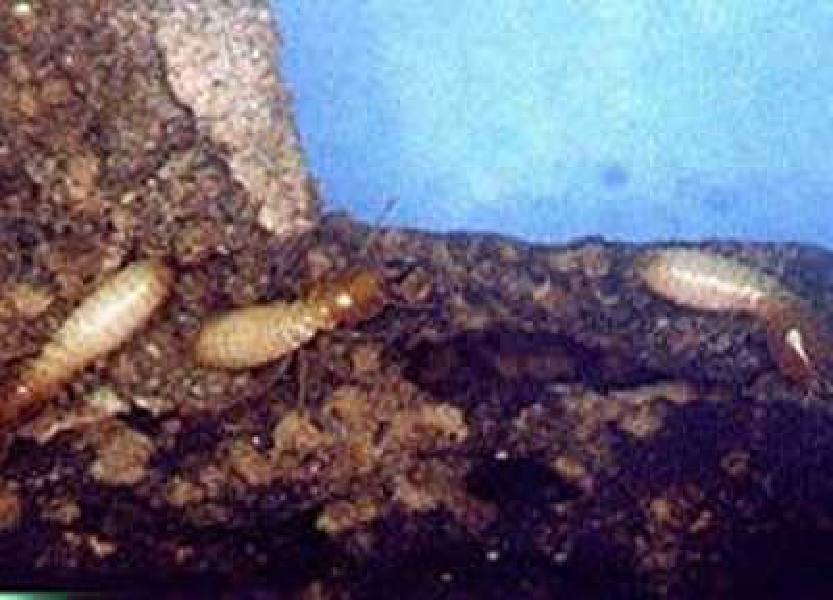
\includegraphics[width=1\textwidth]{Cap1/cupimconcreto}
\caption{Exemplo real de cupim frente ao seu dilema.}
\label{FDII}
\end{figure}

\section{Organiza��o do trabalho}
\subsection{Sub-organiza��o}
O cap�tulo 1 cont�m a introdu��o do trabalho, onde s�o expostos o objetivo, a motiva��o do mesmo, a descri��o do sistema e a formula��o do problema com a nomenclatura utilizada; al�m de uma revis�o bibliogr�fica da literatura relacionada ao tema do trabalho.

\subsubsection{SubSub-organiza��o}

No cap�tulo 2 apresentamos a modelagem din�mica de um manipulador subatuado e o conceito de �ndice de acoplamento para medir o acoplamento din�mico entre as juntas ativas e passivas. Este �ndice � utilizado para a an�lise e projeto de uma metodologia de controle sub�timo do manipulador.

\subsubsection{Outra subsub-organizacao}

O cap�tulo 3 apresenta o controle sub�timo de manipuladores atrav�s de redund�ncia de atua��o. Descreve-se a t�cnica de controle ponto a ponto de manipuladores subatuados. A seguir mostramos  a lineariza��o destes por realimenta��o, cujo efeito � linearizar e desacoplar o sistema n�o linear. Finalmente � proposta uma sequ�ncia de controle sub�timo local das juntas passivas visando a minimiza��o de certos crit�rios como torque, velocidade e em particular a energia consumida pelo sistema. Este � de fato o tema principal deste mestrado.

� tamb�m apresentado no cap�tulo 4 um resumo do projeto de controladores  $H_{2}$ e $H_{\infty}$, cuja principal vantagem � a robustez na presen�a de incertezas param�tricas e dist�rbios externos.

O cap�tulo 5 mostra as caracter�sticas e a opera��o do rob� e do ambiente de simula��o utilizados nos testes e experimenta��o da metodologia apresentada.

Os procedimentos da metodologia e os resultados obtidos para algumas configura��es e diferentes controladores encontram-se no cap�tulo 6.

No cap�tulo 7 s�o apresentadas as conclus�es do trabalho.

Quatro ap�ndices fazem parte do trabalho. O ap�ndice A apresenta alguns t�picos de �lgebra linear que s�o a base do m�todo proposto. No ap�ndice B s�o mostradas as equa��es da matriz de in�rcia e do vetor de torques n�o-inerciais
utilizados na modelagem din�mica do manipulador. No ap�ndice C temos as express�es literais dessas equa��es feitas no software MAPLE e no ap�ndice D alguns programas feitos no software MATLAB utilizados no projeto \cite{Furmento1995}\cite{Morgado2003}.



\chapter{Modelagem Dinâmica de Cupins Cibernéticos}
\section{Modelagem no espa�o das juntas}
Manipuladores subatuados diferem dos totalmente atuados pois s�o equipados com um n�mero de atuadores que � sempre menor que o n�mero de graus de liberdade (GDL). Portanto, nem todos os GDL podem ser controlados ativamente ao mesmo tempo \cite{Sbornian2004}. Por exemplo, com um manipulador planar de 3 juntas equipado com dois atuadores, ou seja, duas juntas ativas e
uma passiva, pode-se controlar ao mesmo tempo duas das juntas a qualquer instante, mas n�o todas. Para controlar todas as juntas de um manipulador subatuado, deve-se usar um controle sequencial. Este princ�pio foi provado pela primeira vez por {arai} usando  argumentos din�micos linearizados \cite{Joea2003}, e � a base para a modelagem no espa�o das juntas e no espa�o Cartesiano. A Tabela \ref{minhatab} apresenta os resultados \cite[p. 50]{Assenmacher1993,Silberschatz1991,Caromel1998}.

\begin{table}
\caption{Exemplo de uma Tabela}
\label{minhatab}

\center
\begin{tabular}{cccc}
  % after \\: \hline or \cline{col1-col2} \cline{col3-col4} ...
  \hline
	Par�metro & Unidade & Valor da simula��o & Valor experimental   \\
	\hline
  Comprimento, $\alpha$ & $m$ &  $8,23$  & $8,54$ \\
  Altura, $\beta$ & $m$     &  $29,1$ & $28,3$\\
	Velocidade, $v$ & $m/s$  &  $60,2$ & $67,3$\\
	\hline
\end{tabular}
\end{table}

Devido ao fato de que no m�ximo $n_{a}$ coordenadas generalizadas (�ngulos das juntas ou vari�veis cartesianas) podem ser controladas num dado instante, o vetor de coordenadas generalizadas � dividido em duas partes, representando as coordenadas generalizadas ativas e as coordenadas generalizadas passivas \cite{Callaghan1995}.

\begin{figure}[ht]
\centering
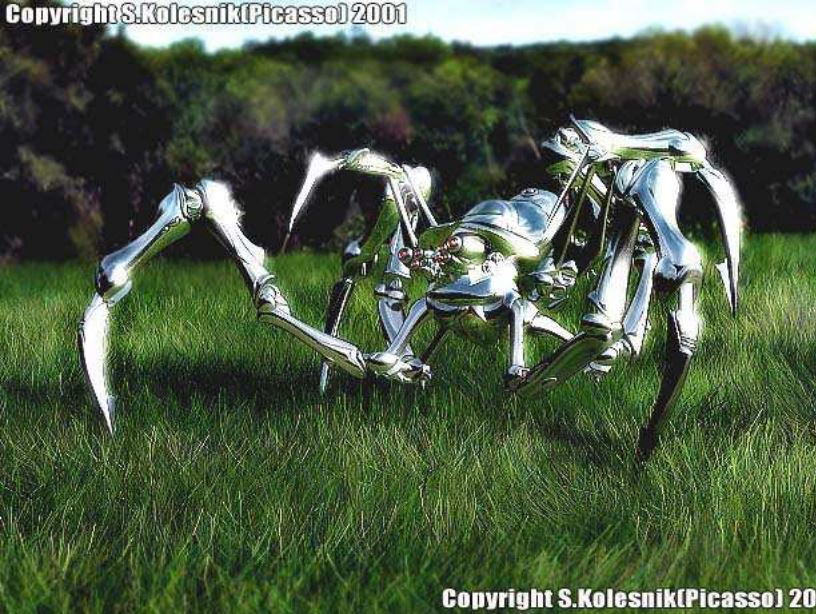
\includegraphics[width=0.75\textwidth]{Cap2/spiderrobot}
\caption{Cupim cibern�tico.}\label{FDIII}
\end{figure}

Considerando um rob� manipulador r�gido, malha aberta, e de $n$-juntas em s�rie. Seja $q$ a representa��o de seu vetor de posi��o angular das juntas  e $\tau$ a representa��o de seu vetor de torque. A equa��o din�mica pelo m�todo de
Lagrange � dada por:
\begin{equation} \label{eq:lagr1}
\frac{d}{dt}(\frac{\partial L}{\partial \dot{q}})-\frac{\partial L}{\partial q}=\tau^{T}.
\end{equation}
O Lagrangiano $L$ � definido como a diferen�a entre as energias cin�tica e potencial do sistema:
\begin{equation} \label{L}
L=T-P
\end{equation}

A energia cin�tica total dos ligamentos � representada:
\begin{equation} \label{energT}
T=\frac{1}{2}\dot{q}^{T}M(q)\dot{q}
\end{equation}


\chapter{Controle Robusto de Concretos Caóticos}
\section{Controle combinado}
Conforme vimos na se��o \ref{ectq3} podemos controlar um sistema nao linear como  atrav�s da t�cnica do torque computado, usando um controlador PD dado por:
\begin{equation} \label{ectq3}
\tau'=\ddot{q}_d+K_v(\dot{q}_d-\dot{q})+K_p(q_d-q) \; ,
\end{equation}
sendo $q_{d}$, $\dot{q}_{d}$ e $\ddot{q}_{d}$ a posi��o desejada, a velocidade desejada e a acelera��o desejada; $K_p$
e $K_v$ s�o matrizes diagonais $n \times n$, sendo que cada elemento da diagonal � um ganho positivo e escalar.

Aqui $M_{est}$ e $b_{est}$ s�o modelos estimados da matriz de in�rcia, $M$, e do vetor de torques n�o inerciais, $b$, do rob� real,  respectivamente. A equa��o de malha fechada do sistema �:
\begin{equation} \label{ectq4}
\ddot{e}+K_v\dot{e}+K_pe=M_{est}^{-1}[(M-M_{est})\ddot{q}+(b-b_{est})] \; .
\end{equation}

Em um manipulador real, podem existir dist�rbios externos tais como atrito, varia��o de torque dos atuadores, e perturba��es em virtude  das cargas no rob�. Se a soma destes dist�rbios for definida como $d_{ext}$ e adicionada � (\ref{ectq4}), teremos
\begin{equation} \label{ectq5}
\ddot{e}+K_v\dot{e}+K_pe=M_{est}^{-1}[(M-M_{est})\ddot{q}+(b-b_{est})+d_{ext}] \; .
\end{equation}


\chapter{Conclusão}
%\section{Conclus�o}

Neste trabalho realizou-se o projeto de uma metodologia de controle sub�timo redundante da junta passiva de um manipulador com tr�s graus de liberdade instantaneamente. Para este prop�sito usou-se nas formula��es o vetor gradiente de uma fun��o escalar que estima o acoplamento entre a junta passiva e as ativas desse manipulador. Aqui a redund�ncia
foi usada da melhor maneira poss�vel sem focalizar o efeito global. Portanto, este m�todo deve ser denominado de \emph{controle �timo local por redund�ncia}. A principal vantagem dessa formula��o � a computa��o em tempo real, que �
necess�ria para o controle do manipulador experimental. Al�m disso esse m�todo pode ser usado com diferentes tipos de controladores, uma vez que as altera��es s�o feitas nas equa��es din�micas do manipulador.

A consequ�ncia direta observada nessa formula��o � a redu��o dos torques na fase de controle da junta passiva, e consequente redu��o da energia el�trica gasta. Isso ocorre devido ao fato de que ao longo da trajet�ria do manipulador
o �ndice de acoplamento de torque tende a ser maximizado, e portanto, menor � o torque necess�rio nos atuadores para se conseguir o posicionamento da junta passiva do manipulador.

Outros resultados indiretos obtidos s�o: um movimento mais uniforme e suave do manipulador e um tempo de acomoda��o menor tanto no posicionamento da junta passiva quanto das ativas, conforme podemos obervar nos gr�ficos de desempenho dos resultados apresentados. Isso ocorre porque a maximiza��o do acoplamento entre as juntas facilita o controle. Assim
ocorrem menos picos de torque, e como as juntas ativas tem ``menos trabalho'' para posicionar a passiva estas se movem menos na dire�ao contr�ria ao movimento daquelas, diminuindo assim as velocidades alcan�adas e os tempos de posicionamento.

Uma extens�o deste trabalho pode ser a implementa��o de um \emph{controle �timo global por redund�ncia} da junta passiva do manipulador. Para isto pode-se fazer o planejamento \emph{off-line} da trajet�ria das juntas de modo a minimizar a energia consumida. Alguns estudos foram feitos nesse sentido, usando o Princ�pio M�nimo de Pontryagin, mas sem resultados satisfat�rios at� o momento.


% REFERENCIAS BIBLIOGRAFICAS
\renewcommand\bibname{\itareferencesnamebabel} %renomear título do capítulo referências

\bibliography{Referencias/referencias}
%\bibliographystyle{abbrvnat}
% Apendices
\appendix
\chapter{Tópicos de Dilema Linear} %opcional
\section{Uma Primeira Se��o para o Ap�ndice}

A matriz de Dilema Linear $M$ e o vetor de torques inerciais $b$,
utilizados na simula��o s�o calculados segundo a formula��o 
abaixo:
\begin{equation}
M=\left[ \begin{array}{ccc}
M_{11} & M_{12} & M_{13} \\
M_{21} & M_{22} & M_{23} \\
M_{31} & M_{32} & M_{33}
\end{array} \right]
\end{equation}

\begin{figure}[h]
\centering
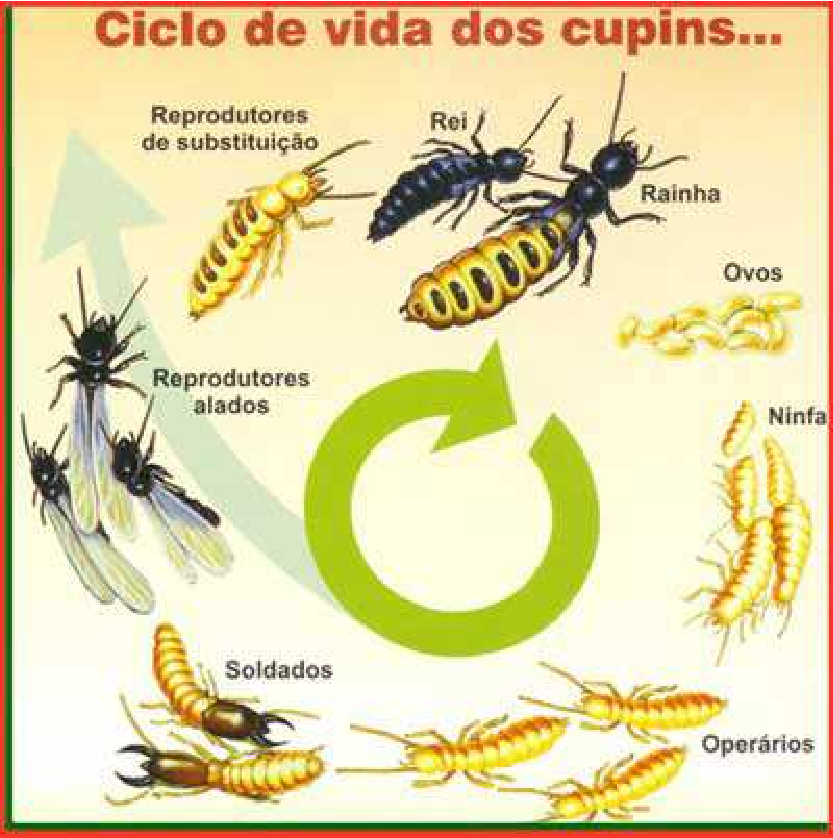
\includegraphics[height=5cm, width=5cm]{ApeA/pragas_ciclo_cupim}
\caption{Uma figura que est� no ap�ndice}\label{FD}
\end{figure}


% Anexos
\annex
\chapter{Exemplo de um Primeiro Anexo} %opcional
% Texto do Primeiro Anexo
\section{Uma Se��o do Primeiro Anexo}
% Texto da primeira secao do primeiro anexo
Algum texto na primeira se��o do primeiro anexo.



% Glossario
%\itaglossary
%\printglossary

% Folha de Registro do Documento
% Valores dos campos do formulario
\FRDitadata{25 de março de 2015}
\FRDitadocnro{DCTA/ITA/DM-018/2015} %(o número de registro você solicita a biblioteca)
\FRDitaorgaointerno{Instituto Tecnológico de Aeronáutica -- ITA}
%Exemplo no caso de pós-graduação: Instituto Tecnol{\'o}gico de Aeron{\'a}utica -- ITA
\FRDitapalavrasautor{Cupim; Cimento; Estruturas}
\FRDitapalavrasresult{Cupim; Dilema; Construção}
%Exemplo no caso de graduação (TG):
%\FRDitapalavraapresentacao{Trabalho de Graduação, ITA, São José dos Campos, 2015. \NumPenultimaPagina\ páginas.}
%Exemplo no caso de pós-graduação (msc, dsc):
\FRDitapalavraapresentacao{ITA, São José dos Campos. Curso de Mestrado. Programa de Pós-Graduação em Engenharia Aeronáutica e Mecânica. Área de Sistemas Aeroespaciais e Mecatrônica. Orientador: Prof.~Dr. Adalberto Santos Dupont. Coorientadora: Prof$^\textnormal{a}$.~Dr$^\textnormal{a}$. Doralice Serra. Defesa em 05/03/2015. Publicada em 25/03/2015.}
\FRDitaresumo{Aqui come�a o resumo do referido trabalho. N�o tenho a menor id�ia do que colocar aqui. Sendo assim, vou inventar. L� vai: Este trabalho apresenta uma metodologia de controle de posi��o das juntas passivas de um manipulador subatuado de uma maneira sub�tima. O termo subatuado se refere ao fato de que nem todas as juntas ou graus de liberdade do sistema s�o equipados com atuadores, o que ocorre na pr�tica devido a falhas ou como resultado de projeto. As juntas passivas de manipuladores desse tipo s�o indiretamente controladas pelo movimento das juntas ativas usando as caracter�sticas de acoplamento da din�mica de manipuladores. A utiliza��o de redund�ncia de atua��o das juntas ativas permite a minimiza��o de alguns crit�rios, como consumo de energia, por exemplo.
Apesar da estrutura cinem�tica de manipuladores subatuados ser id�ntica a do totalmente atuado, em geral suas carater�sticas din�micas diferem devido a presen�a de juntas passivas. Assim, apresentamos a modelagem din�mica de um manipulador subatuado e o conceito de �ndice de acoplamento. Este �ndice � utilizado na sequ�ncia de controle �timo do \mbox{manipulador}.
A hip�tese de que o n�mero de juntas ativas seja maior que o n�mero de
passivas  $(n_{a} > n_{p})$  permite o controle �timo das juntas passivas, uma vez que na etapa de controle destas h� mais entradas (torques nos atuadores das juntas ativas), que elementos a controlar (posi��o das juntas passivas). }
%  Primeiro Parametro: Nacional ou Internacional -- N/I
%  Segundo parametro: Ostensivo, Reservado, Confidencial ou Secreto -- O/R/C/S
\FRDitaOpcoes{N}{O}
% Cria o formulario
\itaFRD

\end{document}
% Fim do Documento. O massacre acabou!!! :-)
